% !TEX root = ../thesis.tex

\chapter{Introduction}
\label{chapter:introgen}

Recent years have seen enormous advances in the field of cosmology. Thanks to technological advancements, wide-field galaxy surveys have helped mapping the universe, in particular provide high-precision data on the distribution of galaxies. From the earliest realisations that these observed galaxies can be used to trace the underlying matter density fields, the field of LSS research has been transformed into a data-driven science. 

Next-generation large-scale surveys will be able to observe at unprecedented precision. The work in this thesis was undertaken in an effort to improve the theoretical description of the statistical models used to interpret these upcoming datasets in an as unbiased manner as possible. To start, in this chapter we introduce the standard cosmological model, $\Lambda$CDM, and briefly discuss the observational evidence supporting the standard model of cosmology. We also discuss structure formation in the universe, and introduce galaxy statistics, which has been the crucial tool for studying the clustering of galaxies in the universe. Up to now, the two-point correlation function, or power spectrum in Fourier space, has been a cosmologist's most reliable statistic describing the LSS and constraining cosmological parameters. We will give a brief overview of what has been achieved with the power spectrum, and introduce the galaxy bispectrum as the first of the higher-order correlation functions. 

Estuans interius ira vehementi

\todo{describe rest of chapters}

\section{The standard cosmological model}

Over the past several decades, a consensus model for describing the evolution of the universe has emerged.  Evidence for this model is provided by a variety of observations, made possible due to technological advancements, such as the measurements of the cosmic microwave background (CMB), distance measurements using Type 1a Supernovae (SNe), and large-scale structure surveys. 

This standard model for the evolution of the universe predicts that approximately 13.8 billion years ago, the universe was in a hot and dense `Big Bang' state, from which it has continued to expand since. From Type 1a SNe measurements, it has been inferred that the late-time expansion of the universe is accelerating due to an energy component referred to as `dark energy', the physical origin of which has not yet been understood, but described by some cosmological constant $\Lambda$. Approximateley 70\% of the universe's energy budget at the present day is comprised of this dark energy. The remaining amount primarily consists of `cold dark matter' (CDM), a collisionless component which makes up about 25\% of the universe's energy content. The small remaining amount is comprised of roughly 4\% of the more familiar baryonic matter, which interacts electromagnetically, and a small relativistic radiation component (photons and neutrinos). See figure~\ref{fig:contentuniverse} for an illustration of the energy components of the universe at present day. It is from these dominant energy components that the colloquial name of the standard cosmological model is derived-- it is referred to as $\Lambda$CDM.
\begin{figure}[ht]
	\centering
	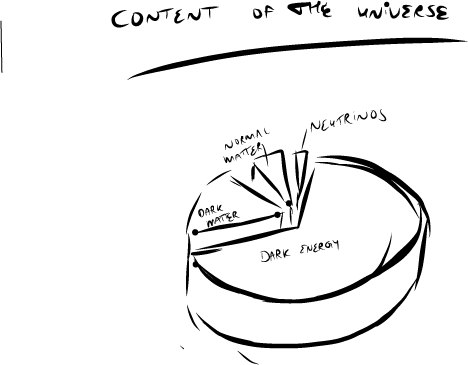
\includegraphics[width=0.6\textwidth]{fig/placeholder_universecontent.png}
	\caption{Picture of content of universe?}
	\label{fig:contentuniverse}
\end{figure}

\begin{figure}[ht]
	\centering
	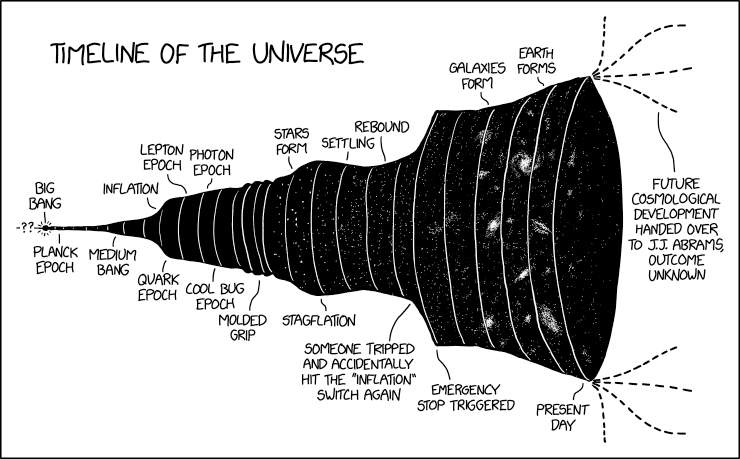
\includegraphics[width=0.6\textwidth]{fig/timeline_of_the_universe.png}
	\caption{Picture of timeline of universe?}
	\label{fig:timelineuniverse}
\end{figure}
In the 1980's, the theory of inflation was coined~\cite{Guth:1980zm,Linde:1981mu,Albrecht:1982wi}, which has since become the prevailing theory for the early universe and its initial conditions. As a theory, it successfully solves the horizon, flatness, homogeneity and isotropy problems. During inflation, the universe is expanding exponentially, rapidly increasing its scale by a factor of at least $\approx 10^{27}$. During this period of exponential expansion, quantum fluctuations are stretched to macroscopic level. These are the seeds of the cosmic structure we observe today. It is worth noting that while the properties of the universe (near homogeneous, isotropic, and spatially flat) as predicted by inflation have been confirmed observationally to very high precision, but as of yet there is no conclusive observational evidence for the inflationary model itself. 

After inflation ends, the universe cooled down, and keeps expanding though at a much slower rate than it did before. The thermal evolution of the universe is defined by the `competition' between the interaction rates of the particles and the expansion rate of the universe itself. The baryonic mass of the universe consists of approximately 75\% hydrogen ions and 25\% helium ions, plus small amounts of deuterium and lithium, all of which are created through Big Bang nucleosynthesis. Electrons, protons, and neutrinos are also present, and the charged baryonic matter is tightly coupled by electromagnetic interaction. Furthermore, the free electrons are tightly coupled also, to the photons, via Thompson scattering. All of this results in the so-called photon-baryon fluid. The pressure of this fluid prevents the fluctuations from gravitationally collapsing, which leads instead to the generation of acoustic waves. These are known as the Baryon Acoustic Oscillations (BAO), propagating until the protons and baryons decouple. This occurs around the time of `recombination' around 400,000 years after the Big Bang. At recombination, the universe has cooled down sufficiently for neutral hydrogen to form, and the now decoupled photons can free stream from the `surface of last scattering' through the universe. This background radiation, the `first light' of the universe, can be observed today and has a temperature of about 2.7 K-- it is known as the Cosmic Microwave Background (CMB), and primordial fluctuation patterns are imprinted on the temperature fluctuations of the CMB. 

Around 50,000 years after the Big Bang, and after a period of radiation domination, the universe becomes dominated by its matter content. This matter dominated era lasts for about 10 billion years. Under matter domination, the primordial density fluctuations grow due to gravitational instability. This gravitational collapse eventually leads to the formation of the cosmic web, which is a non-linear structure formed by halos, voids, and filaments, dominated by CDM. \todo{add picture?} Baryonic matter inside these dark matter halos cools down, collapses, and goes on to form stars and galaxies. Formation of this large scale structure is hierarchical, as smaller objects form first and merge to into larger structures. The resulting evolution of structure can be well-described by a linear description of perturbations on large scales (of about 150Mpc), but the small-scale nonlinearities of the fluctuations pose serious theoretical challenges.

In the standard $\Lambda$CDM model, the universe is assumed to be spatially flat, and its evolution is described by six parameters-- the present-day baryon and cold dark matter densities, the angular size of the sound horizon, the optical depth due to reionisation, the scalar power spectrum index, and the amplitude of the primoridal curvature perturbations. The current best constraints on these parameters are given in table~\ref{tab:planck2018params}.

\begin{table}[ht]
	\centering
\begin{tabular}{ l | l}
	\textbf{Parameter} & \textbf{Value} \\
	\hline
	$\Omega_b h^2$ (baryon density) & $0.02242 \pm 0.00014$ \\
	$\Omega_c h^2$ (CDM density) & $0.11933 \pm 0.00091$ \\
	$100 \theta_\star$ (angular size of sound horizon) & $1.04101 \pm 0.00029$ \\
	$\tau$ (optical depth due to reionisation) & $0.0561 \pm 0.0071$ \\
	$n_s$ (scalar power spectrum index) & $0.9665 \pm 0.0038$ \\
	$\ln (10^{10} A_s)$ (amplitude of primordial curvature perturbations) & $3.047 \pm 0.014$
\end{tabular}
	\caption{Planck 2018 best-fit parameters in the standard, spatially flat, $\Lambda$CDM model~\cite{Aghanim:2018eyx}.} \label{tab:planck2018params}
\end{table}

Support for the $\Lambda$CDM model comes from a variety of observational probes. The anisotropies of the CMB as measured by the WMAP~\cite{Bennett:2013} and Planck~\cite{Aghanim:2018eyx} satellites, and the ground-based telescopes Atacama Cosmology Telescope and South Pole Telescope, which have all supplied strong constraints on matter and radiation densities, the angular diameter distance to the surface of last scattering, and the shape and the amplitude of the primordial power spectrum. The BAO features have been measured successfully by galaxy redshift surveys on scales of about 150 Mpc. This BAO feature is the imprint of the acoustic waves in the baryon-photon fluid onto the clustering of density field tracers. Measurements of the BAO have provided constraints on the expansion rate of the universe across a wide range of different redshifts. \todo{few citations} Furthermore, Type 1a SNe have yielded the first evidence for dark energy~\cite{SupernovaSearchTeam:1998fmf,SupernovaCosmologyProject:1998vns}, as well as complementary constraints on the expansion rate of the universe and the value of the present-day Hubble parameter $H_0$\todo{fix more citations}

\section{Observing large scale structure}

In this section, we will briefly describe the various effects that during the expansion history of the universe have driven the formation of the LSS of the universe, and the observational history thereof. As described in the previous section, the most natural explanation for the formation of the large scale structure of the universe as observed in galaxy surveys is for them to be the result of amplification of the primordial fluctuations due to gravitational interaction of cold dark matter. 

Already before the detailed observations of the CMB anisotropies that reveal the imprint of the stretched-out primordial fluctuations, it was known that the galaxies in our universe are not randomly distributed. The first detections of this structure on larger scales was through a variety of galaxy surveys that aimed to observe and map the distribution of galaxies in the local universe. This all started off with Hubble's first detections of inhomogeneities in the early 20th century, at the time incorrectly thought to be `spiral nebulae'~\cite{Hubble:1926,Hubble:1934}. Following this, advancements in cosmology have been primarily held back by lack of sufficient technological progress to carry out precision surveys at large scales, until the publication of larger galaxy catalogues in the 1960's~\cite{Shane:1967,Zwicky:1961}. Around the same time, theoretical modelling advanced with the realisation that galaxies could be used as biased tracers of the underlying dark matter density field. A series of important papers followed, from systematic analysis of galaxy catalogues~\cite{Peebles:1973} to the first cosmological inferences from LSS data\todo{insert citations}. 

Technological advancements, allowing for larger and more precise datasets, made further theoretical progress possible. Interpretations of clustering results gave rise to a new field of study known as galaxy bias, studying the relationship between the galaxies and the underlying dark matter\todo{add citations}-- a brief overview of the relevant local model of galaxy bias for the purpose of this thesis is given in section~\ref{section:galaxybias} along with appropriate references for further reading. Peculiar velocities of galaxies were found to influence observations of clustering, which lead to several important publications on redshift-space distortions~\cite{Kaiser:1987qv}\todo{add more citations}. These in turn were significant for the early redshift surveys~\cite{Cole:1994wf,Loveday:1995gk,Tadros:1999ky}. The early analyses also provided some of the earliest evidence for the $\Lambda$CDM model, by showing that the then-prevailing theory of a flat, matter-dominated universe did not explain the observed clustering data.

\begin{figure}[ht]
	\centering
	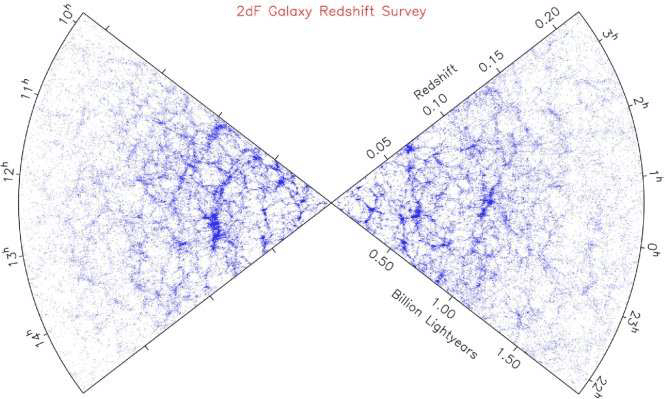
\includegraphics[width=0.8\textwidth]{fig/placeholder_redshiftsurvey.png}
	\caption{Cartoon of redshift survey, find one of eg sdss?}
	\label{fig:redshiftsurveypicture}
\end{figure}

Accurate redshift measurements made possible by the rise of new multi-fiber spectrograph technology allowed for redshift-space mapping of hundreds of thousands of objects. Pioneering surveys in this field are the Two-degree Field Galaxy Redshift Survey (2dFGRS)~\cite{2DFGRS:2001zay} and the Sloan Digital Sky Survey~\cite{SDSS:2000hjo}-- see figure~\ref{fig:redshiftsurveypicture} for an example of the large scale structure as measured by these redshift surveys.

Measurements of the BAO in galaxy clustering surveys can help optimise constraints on the expansion rate and on properties of dark energy. The Baryon Acoustic Oscillation Survey (BOSS)~\cite{Dawson:2012} has yielded a dataset with redshift measurements for more than 1.5 million galaxies, with redshifts ranging from $0.2 < z < 0.75$ which has resulted in percent-level constraints on the expansion rate in this redshift range~\cite{BOSS:2016wmc}. These constraints are complemented at lower redshift by results from the 6dF Redshift Survey~\cite{Beutler:2011} and at higher redshift by the WiggleZ survey~\cite{Blake:2011a,Blake:2011b}. 

There remains a number of unanswered questions in cosmology and LSS, for example finding out more about the origin of cosmic acceleration, and studying the physics of the early universe, which includes detection of primordial non-Gaussianity. Such a detection could help discriminate between various theories of inflation and other models of the early universe. The current state-of-the-art surveys are the so-called Stage III surveys, and they include eBOSS, the Dark Energy Survey (DES), and the Hobby Eberly Telescope Dark Energy Experiment (HETDEX). 
The next-generation surveys, which will provide us with a wealth of high precision cosmological information, are known as Stage IV surveys. These include e.g. the Dark Energy Spectroscopic Instrument (DESI), the Subaru Prime Focus Spectrograph (PFS), 4MOST, and space-based instruments Wide Field Infrared Survey Telescope (WFIRST) and Euclid \todo{add citations, footnote links to websites, and update any names that have got changed}.

In this thesis, we treat two surveys with specific interest. The first is a Stage IV spectroscopic galaxy survey similar to what will be carried out by the Euclid satellite. Secondly, we consider in more detail the use of intensity mapping of 21cm emission as a tracer of the galaxy distribution in cosmology, such as the Square Kilometre Array (SKA), HIRAX and PUMA. These surveys are discussed in more detail in chapter~\ref{chapter:detect}. 


\section{Statistics of galaxy clustering}
\label{section:introbisp} 

Tests of theories of the early universe that describe the primordial fluctuations are statistical in nature for a number of reasons. For one, there is no direct observational access to primordial fluctuations, and secondly, the timescales required to follow cosmological evolution of systems is much longer than that over which observations are realistically possible. In essence this means that observations on the past lightcone show different objects at different phases of their evolution, and as a result, tests of the evolution of large scale structure must be carried out statistically. 

A goal of theoretical cosmology is to make statistical predictions which depend on the statistical properties of primordial perturbations, which in turn lead to the formation of large scale structures in the universe. In these models, the observable universe is modelled simply as a stochastic realisation of a statistical ensemble of possibilities. The most widely considered models are based on the inflationary paradigm, and generically give rise to adiabatic Gaussian initial fluctuations. In this case, the origin of stochasticity lies in quantum fluctuations that were generated in the early universe. 

When observing the LSS of galaxies, we usually compare the observed distribution with the distribution of an unperturbed universe. We measure the fluctuations in the distribution, 
\begin{equation}
	\delta(\x) = \frac{\rho(\x) - \bar{\rho}}{\bar{\rho}}\,,
\end{equation}
where $\bar{\rho}$ is the mean observed galaxy density. 


\section{The two-point function}

A purely Gaussian field is fully described by the two-point correlation function or power spectrum. The two-point correlation function is defined as the joint ensemble average of the density at two different points $\x$ and $\x + \textbf{r}$, i.e. 
\begin{equation}
	\xi(r) = \langle \delta(\x) \delta(\x + \textbf{r}) \rangle,
\end{equation}
which is dependent on the distance $r$ between the two points only, due to statistical homogeneity and isotropy which are assumed throughout. Usually, the density contrast $\delta$ is expressed in terms of its Fourier space components, where our Fourier convention is 

\begin{equation}
	\delta({\x}) = \int \frac{\diff^3k}{(2\pi)^3} \, e^{\i \k \cdot \x } \delta(\x),
\end{equation}
where $\delta(\k)$ are complex random variables. Note that there are generally two Fourier conventions that are used in literature on the galaxy statistics, which lead to a difference of $(2\pi)^3$ in the definition of the power spectrum or two-point function. The other choice of Fourier convention is to reverse where the factor of $(2\pi)^3$ goes in the Fourier transforms, that is, using $f(\x) = \int \diff^3k e^{\i \k \cdot \x} f(\k) $ and $f(\k) = \int \frac{\diff^3 x}{(2\pi)^3} e^{-\i \k \cdot \x} f(\x)$ instead of our convention used here.

Since the density contrast is real, this means that we have
\begin{equation}
	\delta(k) = \delta^*(-\k).
\end{equation}

Similarly, the correlators can also be computed in Fourier space, as follows, 
\begin{equation}
	\langle \delta(\k) \delta(\k') \rangle = \int \diff^3 x \diff^3 r \langle \delta(\x) \delta(\x + \r)\rangle e^{-\i (\k + \k') \cdot \x - \i \k' \cdot \r}.
\end{equation}
This can be rewritten using the definition of the two-point correlation function as 
\begin{equation}
	\langle \delta(\k) \delta(\k') \rangle = \int \diff^3 x \diff^3 r \xi(r) e^{-\i (\k + \k') \cdot \x - \i \k' \cdot \r},
\end{equation}
and, performing one of the integrals, 
\begin{align}
	\langle \delta(\k) \delta(\k') \rangle &= (2\pi)^3 \delta^D(\k + \k') \int \diff^3 r \xi(r) e^{\i \k \cdot \r} \\
	&\equiv (2\pi)^3 \delta^D(\k + \k') P(k),
\end{align}
where $P(k)$ is by definition the density power spectrum.

\subsection{The power spectrum}
\todo[inline]{Power spectrum introduction -- need to take from section above}

\subsection{The angular power spectrum}
\todo[inline]{$C_\ell$ stuff}

\section{The three-point function}

Higher-order correlation functions are defined as the connected part of the joint ensemble average of the density in an arbitrary number of locations. In principle it is possible define any order of correlation function like this, but they will rapidly become more computationally complex and expensive. In the case of a purely Gaussian field, the only non-vanishing connected part is the two-point correlation function. This is a direct consequence of Wick's theorem for Gaussian fields, and has a number of important consequences. Firstly it means that a purely Gaussian, statistically homogeneous and isotropic field is fully described by its two-point correlation function or power spectrum, and secondly it means that the statistical properties of any field, which is not necessarily linear, can be written in terms of combinations of two-point correlation functions -- as long as the field is built from a Gaussian field $\delta$. In a generic form, Wick's theorem can be expressed as 
\begin{align}
	&\langle \delta(\ka) \ldots \delta(\bm{k}_{2p + 1}) \rangle = 0 \nonumber \\
	&\langle \delta(\ka) \ldots \delta(\bm{k}_{2p})\rangle = \sum_{[\text{all distinct pairs}]} \prod_{[p \text{ pairs } (i,j)]} \langle \delta(\bm{k}_i) \delta(\bm{k}_j) \rangle.  
\end{align}

More concretely, this means that for a purely Gaussian field, $\langle \delta(\ka) \delta(\kb) \delta(\kc)\rangle = 0$. However, this changes in the presence of any sources of non-linearity. BLAH. An important consequence of non-linear evolution of structure is that the statistics of odd-number density fields are no longer vanishing. The leading odd-number statistic which will be non-zero in the case of non-linear evolution if the three-point correlation function or the bispectrum in Fourier space, 
\begin{equation}
	\langle \delta(\ka) \delta(\kb) \delta(\kc) \rangle = (2 \pi )^3 \delta^\mathrm{D}(\ka + \kb + \kc) \left[ 2 F_2(\ka,\kb) P_\mathrm{L}(\ka) P_\mathrm{L}(\kb) + \text{ 2 c.p.} \right]
\end{equation}
where $F_2$ is the Fourier space density evolution kernel, $P_\mathrm{L}$ is the linear power spectrum from the previous discussion, and redshift dependence is suppressed for brevity. 

Some blah blah about higher order statistics and their importance in future surveys (higher precision data, non-Gaussianities in the universe and effects that give rise to nonlinearities)

\subsection{The matter bispectrum}

The bispectrum is a non-Gaussian statistic, and as such is especially sensitive to any forms of non-linearity in the universe. It is an essential probe for e.g. primordial non-Gaussianity, though there are also other sources of non-Gaussianities in the universe. Primordial non-Gaussianity, which is often parametrised by the non-linear parameter $\fnl$, is predicted by different types of inflation and other theories of the early universe; meaning that improvement of constraints on $\fnl$ could help discriminate between these theories and help shed light on the very early universe and the seeds of structure formation. 

In this section we will go into more detail as to how various amplitudes and signs of the bispectrum correspond to real-space signatures. The bispectrum in Fourier space forms a closed triangle correlating three different wave-vectors and, unlike the power spectrum or two-point function, is able to correlate different scales. The matter bispectrum is unique from the thus far more well-studied CMB bispectrum in that it is able to form a three-dimensional map of the universe, whereas the cosmic microwave background provides a two-dimensional snapshot of the first light only. It is therefore essential to try and improve the theoretical description of the matter bispectrum if we are to utilise the wealth of information from next-generation high-precision galaxy surveys in as good and as unbiased a manner as possible. 

Where the power spectrum is a measure of probability of, e.g. in the case of the galaxy power spectrum, finding galaxies at distance corresponding to separation of points $r$ from each other, the bispectrum similarly maps this to a probability in a three-dimensional equivalent. That is, it can correspond directly to what we know as the cosmic web, and the galaxy or dark matter distributions therein. The bispectrum has degrees of freedom in both modulus of the wavevector i.e. scales of correlation, as well as the shape of the triangle itself. Different triangle shapes correspond to different real-space bispectrum signatures.

Theoretical blah about the matter bispectrum, definitions, showing how various bispectrum signals translate to real space shapes and modulations of signal

\subsection{Matter bispectrum in observations}

Bispectrum in observation -- can skip over any CMB and just focus on lss

\section{Galaxy bias}
\label{section:galaxybias}


(Very) brief overview of the relevant bias


\section{Primordial non-Gaussianity}

Types of primodial non-Gaussianity in the bispectrum, their signatures on various scales, scale dependence it introduces in the clustering bias etc. 


cum sit enim proprium \\
viro sapienti \\
supra petram ponere \\
sedem fundamenti \\
stultus ego comparor \\
fluvio labenti \\
sub eodem tramite \\
nunquam permanenti 